\documentclass[10pt,a4paper]{article}
\usepackage[a4paper,top=2.0cm,bottom=1.9cm,left=1.7cm,right=1.7cm,headsep=0.5cm]{geometry}
\usepackage{fontspec}
\usepackage{xetexko}
\setmainfont{TeX Gyre Termes}
\setmainhangulfont{Noto Serif CJK KR}
\setmainhanjafont{Noto Serif CJK KR}
\AtBeginDocument{\xetexkofontregime{latin}}
\usepackage{amsmath,amssymb}
\usepackage{chemfig}
\usepackage[version=4]{mhchem}
\usepackage{tabularx,booktabs,array,multirow}
\usepackage{enumitem}
\usepackage{fancyhdr}
\usepackage[most]{tcolorbox}
\usepackage{tikz}
\usetikzlibrary{arrows.meta,decorations.pathmorphing,patterns,calc,shapes.geometric}
\usepackage[hidelinks]{hyperref}

\setlength{\parindent}{0pt}
\linespread{1.08}
\setchemfig{atom sep=1.6em,bond offset=1pt,double bond sep=2.2pt}

\pagestyle{fancy}
\fancyhf{}
\fancyhead[L]{\small CM3191 Organic --- Expt.\ 4 (Part 1) --- Grignard: ($\pm$)-Linalool}
\fancyhead[R]{\small KIM DONGHWAN $\bullet$ B7 $\bullet$ Thu}
\fancyfoot[C]{\small\thepage}
\renewcommand{\headrulewidth}{0.4pt}
\fancypagestyle{official}{\fancyhf{}\fancyhead[L]{CM3191}\fancyhead[R]{27}\renewcommand{\headrulewidth}{0pt}}

\newcommand{\pagetitle}[3]{%
  \begin{center}
  {\Large\bfseries #1}\\[3pt]
  {\large #2}\\[4pt]
  {\footnotesize #3}
  \end{center}\vspace{-4pt}\noindent\rule{\textwidth}{0.8pt}\vspace{4pt}}
\newcommand{\sect}[1]{\par\medskip{\large\bfseries #1}\par\smallskip}
\newcommand{\sub}[1]{\par\smallskip{\bfseries #1}\par\vspace{2pt}}
\newcommand{\why}[1]{\par\vspace{1pt}{\footnotesize\textit{Why:} #1}}
\newcommand{\iyu}[1]{\par\vspace{1pt}{\footnotesize\textit{이유:} #1}}
\newcommand{\confirm}[1]{\textbf{[CONFIRM: #1]}}
\newcommand{\bx}{$\square$}
\newlist{bench}{enumerate}{1}
\setlist[bench]{label={$\square$\ \arabic*.},leftmargin=3.0em,labelsep=0.4em,itemsep=2pt,parsep=0pt,topsep=2pt}
\newcolumntype{Y}{>{\raggedright\arraybackslash}X}
\newcommand{\fillbox}[1]{\rule{0pt}{#1}}

\tcbset{safety/.style={enhanced,colback=white,colframe=black,boxrule=0.6pt,arc=0pt,left=5pt,right=5pt,top=4pt,bottom=4pt,fonttitle=\bfseries,coltitle=black,colbacktitle=white,attach title to upper,after title={\par\smallskip}}}

\begin{document}

%%%%%%%%%%%%%%%%%%%%%%%%%%%%%%%%%%%%%%%%%%%%%%%%%%%%%%%%%%%%%%%%%%%%%%%%%%%%%%%%
% PAGE 1 -- PRE-LAB CHECKLIST
%%%%%%%%%%%%%%%%%%%%%%%%%%%%%%%%%%%%%%%%%%%%%%%%%%%%%%%%%%%%%%%%%%%%%%%%%%%%%%%%
\pagetitle{ORGANIC EXPERIMENT 4, PART 1 --- PRE-LAB CHECKLIST}
{Synthesis of ($\pm$)-Linalool by Grignard Addition on a Schlenk Line}
{Condensed from the CM3191 Organic Lab Manual AY26/27 (Dr Hoang T.\,G., pp.\ 19--24, 27) and lecture CM3191 Org L4.\\ Week 9, \textbf{Thursday 15 October 2026}, Thursday lab (Dr Hoang T.\,G.), \textbf{Group A} (Schlenk line this week; reduction in Week 10). Venue \confirm{not stated in the organic schedule}.}

\begin{center}
\begin{tabular}{@{}c c c c c@{}}
\chemfig{-[:30](=[:90]O)-[:-30]-[:30]-[:-30]=[:30](-[:90])-[:-30]} &
\raisebox{10pt}{$+$} &
\raisebox{8pt}{\chemfig{=[:30]-[:-30]MgBr}} &
\raisebox{14pt}{$\xrightarrow[\text{\scriptsize then sat.\ NH$_4$Cl (aq)}]{\text{\scriptsize THF, 0\,°C $\to$ RT, 90 min}}$} &
\chemfig{=[:30]-[:-30](-[:90]OH)(-[:-90])-[:30]-[:-30]-[:30]=[:-30](-[:-90])-[:30]}\\[2pt]
{\footnotesize 6-methyl-5-hepten-2-one} & & {\footnotesize vinylMgBr} & & {\footnotesize ($\pm$)-linalool}\\
{\footnotesize 0.44 mL, 2.98 mmol} & & {\footnotesize 1 M in THF, 7.5 mL (2.5 equiv)} & & {\footnotesize 0.460 g theor.}\\
\end{tabular}
\end{center}

\sect{1. Reagent table (manual values; blanks in the manual filled by calculation)}
{\small
\begin{tabularx}{\textwidth}{@{}l c c c c c Y@{}}
\toprule
\textbf{Reagent} & \textbf{MW / conc.} & \textbf{Density} & \textbf{Amount} & \textbf{mmol} & \textbf{Equiv.} & \textbf{Role}\\
\midrule
6-Methyl-5-hepten-2-one & 126.20 & 0.855 g/mL & 0.44 mL (0.376 g) & 2.98 & 1.00 & ketone (limiting)\\
Vinylmagnesium bromide & 131.25; 1.0 M in THF & --- & 7.5 mL & 7.5 & 2.52 & nucleophile\\
THF (anhydrous) & 72.11 & --- & 5 mL & --- & --- & solvent\\
Sat.\ NH$_4$Cl (aq) & --- & --- & 10 mL & --- & --- & quench\\
\textbf{($\pm$)-Linalool} & 154.25 & --- & \textbf{0.460 g (theor.)} & 2.98 & --- & product\\
\bottomrule
\end{tabularx}}
\par\smallskip
{\footnotesize The manual's table rounds the ketone to 3.0 mmol; from 0.44 mL $\times$ 0.855 g/mL it is 2.98 mmol. Reaction volume $\approx$ 12.9 mL in a 50 mL flask.\\
Recalculate with your actual volume:\quad $m_\text{theor} = V_\text{ketone}\times 0.855\times(154.25/126.20) = \mathbf{1.045\,\boldsymbol{V}_\text{ketone}}$ (g, with $V$ in mL).}

\sect{2. Bring / prepare before the session}
{\small
\begin{tabularx}{\textwidth}{@{}YY@{}}
\bx\ Official datasheet (p.\ 6 here = manual p.\ 27), \textbf{printed} & \bx\ This bench sheet (pp.\ 2--7)\\
\bx\ Lab coat, safety goggles, nitrile gloves, covered shoes & \bx\ Phone for photos of every volume and balance reading\\
\bx\ Ruler + pencil: TLC plate must be \textbf{drawn with distances (cm)} & \bx\ Marker and labels for the crude flask (kept to Week 11)\\
\bx\ Re-read L4: stopcock positions, \textbf{slow} backfill (bubbler suck-back) & \bx\ Know: \textbf{no flammables in the hood} while the heat gun is on\\
\bx\ Schlenk-line port \confirm{assigned port; whether shared with D1} & \bx\ Crude storage until Week 11 \confirm{where and how}\\
\end{tabularx}}

\sect{3. Session timeline (estimate)}
{\small
\begin{tabularx}{\textwidth}{|c|Y|r|}
\hline
\textbf{\#} & \textbf{Stage} & \textbf{Approx.\ time}\\ \hline
1 & Connect two-neck flask to the line; heat-gun drying under vacuum, cool, backfill N$_2$ ($\times$2) & 20 min\\ \hline
2 & Add ketone + anhydrous THF; cool in ice-water bath & 15 min\\ \hline
3 & Purge syringe, withdraw 7.5 mL vinylMgBr under N$_2$, add dropwise & 15 min\\ \hline
4 & Stir at RT --- \emph{meanwhile: quench syringe, pre-weigh 250 mL rbf, set up TLC chamber and separatory funnel} & \textbf{90 min (fixed)}\\ \hline
5 & Quench with sat.\ NH$_4$Cl (ice bath); extract EtOAc $\times$3; brine wash & 30 min\\ \hline
6 & Dry over Na$_2$SO$_4$ (15 min) and run TLC (KMnO$_4$) at the same time & 20 min\\ \hline
7 & Filter, rotary-evaporate, weigh crude; store for Week 11; datasheet photo check and GTA signature & 25 min\\ \hline
\end{tabularx}}

\medskip
\begin{tcolorbox}[safety,title={SAFETY --- from the manual (pp.\ 20--23) and L4}]
\footnotesize
6-Methyl-5-hepten-2-one is a flammable liquid and an eye irritant. Vinylmagnesium bromide is toxic, causes skin irritation and serious eye damage, and \textbf{releases flammable gas with water}. Linalool is a skin and eye irritant. Silica gel is toxic if inhaled (Week 11). Ethyl acetate, THF and diethyl ether are highly flammable; hexane is flammable and a neurotoxin. The \textbf{hot air gun reaches 300--500\,°C}: no flammable chemicals or solvents in the fume hood while heating. Be careful with needles; used syringes go in the \textbf{sharps bin} after the residual Grignard is quenched (sat.\ NH$_4$Cl, waste fume hood; ethylene forms). L4: backfill an evacuated flask \textbf{slowly} so bubbler oil is not sucked into the line; never pull air through a liquid-N$_2$ cold trap (liquid O$_2$ risk).\\
\textbf{Added notes (not in the manual).} The excess Grignard ($\approx$4.5 mmol) releases roughly \textbf{110 mL of ethylene} when quenched, and the quench is exothermic: do not quench in a sealed flask --- remove or vent the septum first and add NH$_4$Cl dropwise in the ice bath. Vent the separatory funnel often (EtOAc). Waste: aqueous layers (Mg salts) $\to$ aqueous waste; EtOAc / THF $\to$ non-halogenated organic waste; needles $\to$ sharps. \confirm{waste bins in the organic lab}
\end{tcolorbox}

%%%%%%%%%%%%%%%%%%%%%%%%%%%%%%%%%%%%%%%%%%%%%%%%%%%%%%%%%%%%%%%%%%%%%%%%%%%%%%%%
% PAGES 2-3 -- BENCH MANUAL (ENGLISH)
%%%%%%%%%%%%%%%%%%%%%%%%%%%%%%%%%%%%%%%%%%%%%%%%%%%%%%%%%%%%%%%%%%%%%%%%%%%%%%%%
\newpage
\begingroup\linespread{1.0}\selectfont
\pagetitle{BENCH MANUAL (ENGLISH)}{Grignard Reaction, Part 1: Reaction, Work-up and TLC}
{Tick each box as you complete the step. ``Why'' notes explain the purpose; they are not extra steps. Column chromatography is Part 2 (Week 11).}

\sub{1.1 Drying the apparatus on the Schlenk line (Appendix A, panel 1)}
\begin{bench}[series=en]
\item Clear the fume hood of \textbf{all flammable chemicals and solvents}. \emph{The heat gun reaches 300--500\,°C.}
\item Put a stir bar in a \textbf{50 mL two-necked rbf}. Fit the \textbf{side neck with a rubber septum}; connect the \textbf{vertical neck to a stopcock adapter} on the Schlenk line. Check that N$_2$ is bubbling through the bubbler.
\item Turn the two-way valve to \textbf{vacuum}. Heat the flask all over with the \textbf{hot air gun} to drive out moisture.
\why{a thin film of water on glass destroys the Grignard reagent (RMgBr + H$_2$O $\to$ RH + Mg(OH)Br) and lowers the yield.}
\item Let the flask cool for a few minutes under vacuum, then turn the valve to \textbf{N$_2$ --- slowly}, watching the bubbler.
\why{opening an evacuated flask too fast pulls bubbler oil back into the manifold (L4).}
\item \textbf{Repeat once more}: vacuum + heat gun $\to$ cool $\to$ N$_2$. \confirm{the manual gives 2 cycles; L4 recommends 3 vacuum--refill cycles}
\item Let the flask cool to \textbf{room temperature} before adding any chemicals.
\end{bench}

\sub{1.2 Reaction}
\begin{bench}[resume*=en]
\item Add \textbf{0.44 mL 6-methyl-5-hepten-2-one} (3 mmol) and \textbf{5 mL anhydrous THF} to the flask. Photograph the volumes. Cool in an \textbf{ice-water bath for 5--10 min}.
\item Clamp the \textbf{vinylMgBr bottle} (1 M in THF) on a retort stand and put it \textbf{under N$_2$} (balloon or Schlenk line).
\item \textbf{Purge a 20 mL syringe with long needle} with N$_2$ (L4: three times).
\item Withdraw \textbf{7.5 mL} of the Grignard solution. \textbf{Before pulling the needle out of the bottle, draw in a little N$_2$.}
\why{the N$_2$ plug protects the reagent at the needle tip from air and stops it dripping during the transfer.}
\item Add the vinylMgBr \textbf{dropwise} through the septum into the cooled, stirred flask. Record start and end times.
\why{the addition is exothermic; slow addition at 0\,°C favours attack on C=O over deprotonation of the $\alpha$-H (the enolate returns ketone on work-up).}
\item \textbf{Remove the ice bath}; stir at room temperature for \textbf{90 min}. Start the timer and record the time.
\item While it stirs: \textbf{quench the residual Grignard} in the syringe and needle with sat.\ NH$_4$Cl \textbf{in the waste fume hood} (ethylene forms); syringe $\to$ \textbf{sharps bin}. Pre-weigh a dry \textbf{250 mL rbf}; set up the TLC chamber (hexane:EtOAc \textbf{9:1}) and separatory funnel.
\end{bench}

\sub{2. Work-up}
\begin{bench}[resume*=en]
\item Turn the two-way valve to \textbf{OFF}; disconnect the flask; close it with rubber septa; take it back to \textbf{your own fume hood}.
\item Cool the flask in an \textbf{ice-water bath}. Add \textbf{10 mL sat.\ NH$_4$Cl dropwise}. \emph{Vent first (not in the manual): about 110 mL of ethylene forms.}
\why{NH$_4$Cl is a weak acid: it protonates the magnesium alkoxide to give linalool and destroys excess vinylMgBr. A strong acid is avoided because linalool is a tertiary allylic alcohol that easily loses water or rearranges under acid.}
\item Add \textbf{10 mL water}; transfer the mixture to a \textbf{150 mL separatory funnel}. Rinse the flask with \textbf{20 mL EtOAc} and add the rinse to the funnel.
\item Shake (vent often) and separate. Collect the \textbf{aqueous} and \textbf{organic} layers in separate conical flasks. \emph{EtOAc (0.90 g/mL) is the top layer.}
\item Return the aqueous layer to the funnel; extract \textbf{2 more times with 20 mL EtOAc} (3 extractions in total). Combine the EtOAc layers ($\approx$60 mL).
\item Return the combined organic layer to the funnel; wash with \textbf{15 mL brine}. Put the organic layer in a \textbf{dry 250 mL conical flask}.
\why{brine pulls dissolved water out of the EtOAc, so the drying agent has less to do.}
\item Add \textbf{anhydrous Na$_2$SO$_4$}; let stand \textbf{15 min}.
\item \textbf{TLC} (while drying): spot the \textbf{starting ketone} and the \textbf{reaction mixture} (from the drying solution). Elute with \textbf{hexane:EtOAc 9:1}; stain with \textbf{KMnO$_4$}. Draw the plate with all distances (cm).
\why{neither compound is UV-active, but both have a C=C that KMnO$_4$ oxidises (yellow-brown spot on purple). The alcohol should run lower than the ketone. This plate sets the eluent for the Week-11 column.}
\item Filter into the \textbf{pre-weighed 250 mL rbf}; remove the solvent on the \textbf{rotary evaporator} $\to$ crude linalool.
\item Weigh \textbf{rbf + crude}; photograph; fill in the \textbf{crude product} section of the datasheet (p.\ 27).
\item Label and store the crude for Week 11. \confirm{storage location; stoppered or under N$_2$}
\item Show photos to the GTA; get the \textbf{printed official datasheet} checked/signed. \confirm{sign now, or after the purified mass in Week 11}
\end{bench}

%%%%%%%%%%%%%%%%%%%%%%%%%%%%%%%%%%%%%%%%%%%%%%%%%%%%%%%%%%%%%%%%%%%%%%%%%%%%%%%%
% PAGES -- BENCH MANUAL (KOREAN)
%%%%%%%%%%%%%%%%%%%%%%%%%%%%%%%%%%%%%%%%%%%%%%%%%%%%%%%%%%%%%%%%%%%%%%%%%%%%%%%%
\endgroup
\newpage
\begingroup\linespread{1.0}\selectfont
\pagetitle{실험 매뉴얼 (한국어)}{Grignard 반응 1부: 반응, 후처리, TLC}
{단계를 마칠 때마다 체크하세요. ``이유''는 목적 설명이며 추가 단계가 아닙니다. 컬럼 크로마토그래피는 2부(11주차)입니다.}

\sub{1.1 Schlenk line에서 장치 건조 (부록 A, 그림 1)}
\begin{bench}[series=kr]
\item 후드 안의 \textbf{인화성 시약과 용매를 모두 치웁니다}. \emph{열풍기(hot air gun)는 300--500\,°C까지 올라갑니다.}
\item \textbf{50 mL 2구 둥근바닥 플라스크}에 교반 막대를 넣습니다. \textbf{옆 입구는 고무 셉텀}으로 막고, \textbf{수직 입구는 Schlenk line의 stopcock adapter}에 연결합니다. 버블러로 N$_2$가 나오고 있는지 확인합니다.
\item 2방향 밸브를 \textbf{진공}으로 돌리고, \textbf{열풍기}로 플라스크 전체를 가열해 수분을 날립니다.
\iyu{유리 표면의 얇은 물막이 Grignard 시약을 분해합니다(RMgBr + H$_2$O $\to$ RH + Mg(OH)Br). 그만큼 수율이 떨어집니다.}
\item 진공 상태로 몇 분 식힌 뒤, 버블러를 보면서 밸브를 \textbf{N$_2$로 천천히} 돌립니다.
\iyu{진공인 플라스크를 너무 빨리 열면 버블러 오일이 매니폴드로 빨려 들어갑니다(L4).}
\item \textbf{한 번 더 반복}합니다: 진공 + 열풍기 $\to$ 식힘 $\to$ N$_2$. \confirm{매뉴얼은 2회, L4 강의는 3회 권장}
\item 시약을 넣기 전에 플라스크를 \textbf{실온까지} 식힙니다.
\end{bench}

\sub{1.2 반응}
\begin{bench}[resume*=kr]
\item 플라스크에 \textbf{6-methyl-5-hepten-2-one 0.44 mL}(3 mmol)와 \textbf{무수 THF 5 mL}를 넣습니다. 부피는 사진으로 남깁니다. \textbf{얼음물 수조에서 5--10분} 식힙니다.
\item \textbf{vinylMgBr 병}(THF 중 1 M)을 스탠드에 고정하고 \textbf{N$_2$ 아래}에 둡니다(풍선 또는 Schlenk line).
\item 긴 바늘을 끼운 \textbf{20 mL 주사기를 N$_2$로 퍼지}합니다(L4: 3회).
\item Grignard 용액 \textbf{7.5 mL}를 뽑습니다. \textbf{바늘을 병에서 빼기 전에 N$_2$를 조금 더 빨아들입니다.}
\iyu{N$_2$ 마개가 바늘 끝의 시약을 공기로부터 보호하고, 옮기는 동안 방울이 떨어지지 않게 합니다.}
\item vinylMgBr를 셉텀을 통해 식혀 둔 교반 중인 플라스크에 \textbf{한 방울씩} 넣습니다. 시작과 끝 시각을 기록합니다.
\iyu{첨가는 발열 반응입니다. 0\,°C에서 천천히 넣어야 $\alpha$-H를 떼는 반응(에놀화, 후처리 후 케톤으로 돌아감)보다 C=O 첨가가 우세합니다.}
\item \textbf{얼음 수조를 치우고} 실온에서 \textbf{90분} 교반합니다. 타이머를 켜고 시각을 기록합니다.
\item 교반하는 동안: 주사기와 바늘에 남은 Grignard를 \textbf{폐액 후드에서} 포화 NH$_4$Cl로 \textbf{quench}합니다(에틸렌 발생). 주사기는 \textbf{sharps 통}에 버립니다. 마른 \textbf{250 mL 둥근바닥 플라스크 무게}를 재 두고, TLC 전개조(헥세인:EtOAc \textbf{9:1})와 분별 깔때기를 준비합니다.
\end{bench}

\sub{2. 후처리}
\begin{bench}[resume*=kr]
\item 2방향 밸브를 \textbf{OFF}로 돌리고 플라스크를 분리합니다. 고무 셉텀으로 막아 \textbf{본인 후드}로 가져옵니다.
\item 플라스크를 \textbf{얼음물 수조}에 넣고 \textbf{포화 NH$_4$Cl 10 mL를 한 방울씩} 넣습니다. \emph{먼저 셉텀을 열거나 벤트하세요(매뉴얼에 없음): 에틸렌이 약 110 mL 나옵니다.}
\iyu{NH$_4$Cl은 약산이라 마그네슘 알콕사이드를 양성자화해 linalool을 만들고, 남은 vinylMgBr를 분해합니다. 강산을 쓰지 않는 이유는 linalool이 3차 알릴 알코올이어서 산에서 쉽게 탈수되거나 재배열되기 때문입니다.}
\item \textbf{물 10 mL}를 넣고 \textbf{150 mL 분별 깔때기}로 옮깁니다. 플라스크를 \textbf{EtOAc 20 mL}로 헹궈 깔때기에 더합니다.
\item 흔들고(자주 벤트) 층을 나눕니다. \textbf{수층}과 \textbf{유기층}을 각각 다른 삼각플라스크에 받습니다. \emph{EtOAc(0.90 g/mL)가 위층입니다.}
\item 수층을 다시 깔때기에 넣고 \textbf{EtOAc 20 mL로 2회 더} 추출합니다(총 3회). EtOAc 층을 합칩니다(약 60 mL).
\item 합친 유기층을 깔때기에 넣고 \textbf{브라인 15 mL}로 씻습니다. 유기층을 \textbf{마른 250 mL 삼각플라스크}에 받습니다.
\iyu{브라인이 EtOAc에 녹아 있는 물을 끌어내서, 건조제가 처리할 물이 줄어듭니다.}
\item \textbf{무수 Na$_2$SO$_4$}를 넣고 \textbf{15분} 둡니다.
\item 건조하는 동안 \textbf{TLC}: \textbf{출발 케톤}과 \textbf{반응 혼합물}(건조 중인 용액)을 점적합니다. \textbf{헥세인:EtOAc 9:1}로 전개하고 \textbf{KMnO$_4$}로 염색합니다. 판 그림에 모든 거리(cm)를 적습니다.
\iyu{두 화합물 모두 UV로는 잘 안 보이지만 C=C가 있어 KMnO$_4$에 산화됩니다(보라 바탕에 노란 갈색 점). 알코올이 케톤보다 아래에 올 것으로 예상됩니다. 이 판으로 11주차 컬럼 용리액을 정합니다.}
\item \textbf{무게를 재 둔 250 mL 둥근바닥 플라스크}에 거르고 \textbf{회전증발기}로 용매를 제거합니다 $\to$ linalool 조생성물.
\item \textbf{플라스크 + 조생성물} 무게를 재고 사진을 찍은 뒤 datasheet(p.\ 27)의 \textbf{crude product} 칸을 채웁니다.
\item 11주차까지 보관할 수 있도록 라벨을 붙여 보관합니다. \confirm{보관 장소; 마개만 할지 N$_2$ 아래 둘지}
\item 사진을 GTA에게 보여 주고 \textbf{인쇄한 공식 datasheet}에 확인/서명을 받습니다. \confirm{지금 서명인지, 11주차 정제 후 서명인지}
\end{bench}

%%%%%%%%%%%%%%%%%%%%%%%%%%%%%%%%%%%%%%%%%%%%%%%%%%%%%%%%%%%%%%%%%%%%%%%%%%%%%%%%
% DATASHEET -- WORKING LOG
%%%%%%%%%%%%%%%%%%%%%%%%%%%%%%%%%%%%%%%%%%%%%%%%%%%%%%%%%%%%%%%%%%%%%%%%%%%%%%%%
\endgroup
\newpage
\pagetitle{DATASHEET --- WORKING LOG}{Synthesis of ($\pm$)-Linalool, Part 1 (Grignard reaction, work-up, TLC)}
{Name: KIM DONGHWAN \qquad Lab group: A \qquad Fumehood: \underline{\hspace{2.2cm}} \qquad Date: 15 Oct 2026 \qquad Photos taken: \bx}

\sub{1. Starting materials}
{\small\renewcommand{\arraystretch}{1.9}
\begin{tabularx}{\textwidth}{|Y|Y|}
\hline
6-Methyl-5-hepten-2-one (mL) & mass = $V\times0.855$ (g)\\ \hline
$n$(ketone) = mass/126.20 (mmol) & VinylMgBr solution (mL)\\ \hline
$n$(vinylMgBr) = $V\times1.0$ M (mmol) & Equiv.\ vinylMgBr\\ \hline
Anhydrous THF (mL) & Theoretical (g) = $1.045\,V_\text{ketone}$\\ \hline
\end{tabularx}}

\sub{2. Crude product (datasheet p.\ 27, ``Crude product'')}
{\small\renewcommand{\arraystretch}{1.9}
\begin{tabularx}{\textwidth}{|Y|Y|}
\hline
Empty 250 mL rbf (g) & rbf + crude (g)\\ \hline
Crude product (g) & Crude mass / theoretical (\%) --- \emph{not a yield}\\ \hline
\end{tabularx}}
\par\smallskip{\footnotesize The crude still contains EtOAc and side products; the true yield comes from the purified mass in Week 11.}

\sub{3. Time log}
{\small\renewcommand{\arraystretch}{1.3}
\begin{tabularx}{\textwidth}{|Y|Y|Y|Y|Y|}
\hline
Drying cycle 1 done & Drying cycle 2 done & Ketone + THF added & Grignard addition start & Addition end\\ \hline
\fillbox{0.9cm} & & & & \\ \hline
Ice bath off (90 min starts) & NH$_4$Cl quench start & Na$_2$SO$_4$ added & TLC run & Rotavap done\\ \hline
\fillbox{0.9cm} & & & & \\ \hline
\end{tabularx}}

\sub{4. Checkpoints}
{\footnotesize\renewcommand{\arraystretch}{1.55}
\begin{tabularx}{\textwidth}{|p{3.4cm}|p{6.3cm}|Y|c|}
\hline
\textbf{Stage} & \textbf{Expected} [source] & \textbf{Observed / time} & \checkmark\\ \hline
Heat-gun drying & no flammables in hood [M]; no visible condensation on glass [E] & & \\ \hline
N$_2$ backfill & bubbler keeps bubbling; no oil sucked back [L] & & \\ \hline
Ketone + THF & clear, colourless solution [E] & & \\ \hline
VinylMgBr in syringe & \emph{record colour}; only the N$_2$ buffer, no air bubbles [E] & & \\ \hline
During addition & \emph{record any warming, colour change or cloudiness} [E] & & \\ \hline
After 90 min at RT & \emph{record colour and any solid (Mg alkoxide)} [E] & & \\ \hline
NH$_4$Cl quench & gas forms (ethylene from excess Grignard) [M]; $\approx$110 mL [C]; warming; white Mg salts [E] & & \\ \hline
Separatory funnel & two layers, EtOAc on top [E] & & \\ \hline
Na$_2$SO$_4$ & some crystals stay free-flowing (solution dry) [E] & & \\ \hline
TLC, KMnO$_4$ & new spot below the ketone; ketone spot faint/absent if complete [E] & & \\ \hline
Crude after rotavap & colourless to pale-yellow oil [E] & & \\ \hline
\end{tabularx}}
\par\smallskip
{\footnotesize Sources: [M] stated in the lab manual; [L] lecture L4; [C] calculated from manual quantities; [E] general expectation, not stated in the manual. The Expected column is a \textbf{checkpoint, not an answer}: record what you actually see; a mismatch is a result worth discussing.}

\newpage
\sub{5. TLC record (hexane:EtOAc 9:1, KMnO$_4$ stain) --- draw the plate and label all distances (cm)}
\begin{center}
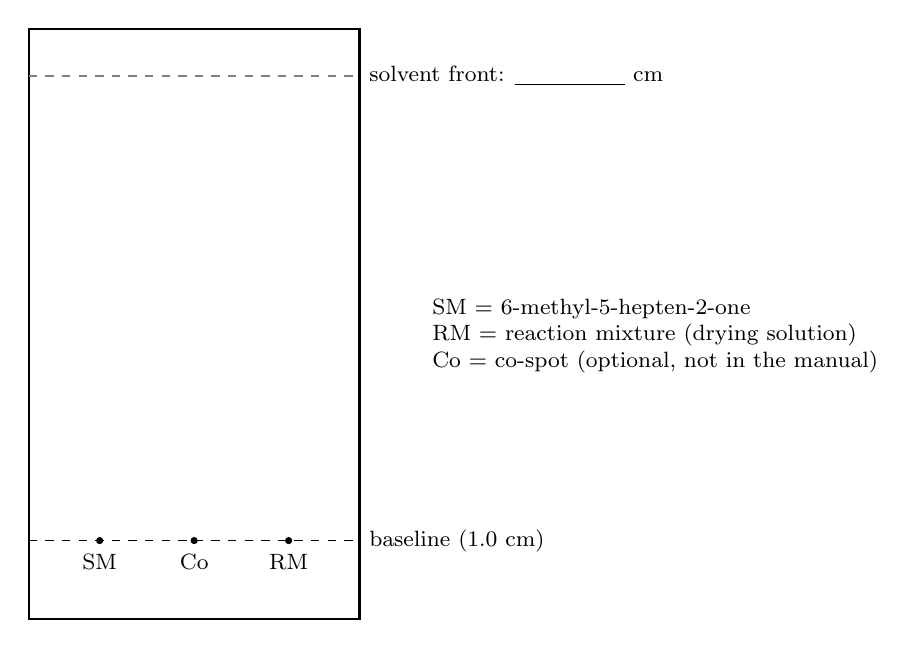
\begin{tikzpicture}
  \draw[thick] (0,0) rectangle (4.2,7.5);
  \draw[dashed] (0,1.0) -- (4.2,1.0) node[right,font=\footnotesize] {baseline (1.0 cm)};
  \draw[dashed,gray] (0,6.9) -- (4.2,6.9) node[right,font=\footnotesize,black] {solvent front: \underline{\hspace{1.4cm}} cm};
  \foreach \x/\l in {0.9/SM,2.1/Co,3.3/RM} {\fill (\x,1.0) circle (1.3pt); \node[below,font=\footnotesize] at (\x,0.95) {\l};}
  \node[font=\footnotesize,align=left,anchor=west] at (5.0,3.6) {SM = 6-methyl-5-hepten-2-one\\ RM = reaction mixture (drying solution)\\ Co = co-spot (optional, not in the manual)};
\end{tikzpicture}
\end{center}
{\small\renewcommand{\arraystretch}{1.7}
\begin{tabularx}{\textwidth}{|l|Y|Y|Y|Y|}
\hline
\textbf{Lane} & \textbf{Spot distance (cm)} & \textbf{Solvent front (cm)} & $\boldsymbol{R_f}$ & \textbf{Colour / intensity}\\ \hline
SM & & & & \\ \hline
RM, spot 1 & & & & \\ \hline
RM, spot 2 & & & & \\ \hline
Co-spot & & & & \\ \hline
\end{tabularx}}

\sub{6. Carry-over to Week 11 (column chromatography)}
{\small\renewcommand{\arraystretch}{1.7}
\begin{tabularx}{\textwidth}{|Y|Y|}
\hline
Crude stored at / label & Product $R_f$ to target in the column\\ \hline
Column eluent (manual): 200 mL hexane:EtOAc 9:1 & Bring: this TLC record + the crude flask\\ \hline
\end{tabularx}}

\sub{7. Other observations}
\vspace{2.6cm}
\noindent\rule{\textwidth}{0.4pt}

\medskip
{\small\renewcommand{\arraystretch}{1.6}
\begin{tabularx}{\textwidth}{|Y|Y|Y|}
\hline
\multicolumn{3}{|l|}{\textbf{To be completed at the end of the session}}\\ \hline
Student signature & GTA name & GTA signature\\ \hline
\fillbox{1.0cm} & & \\ \hline
\end{tabularx}}
\par\medskip
{\footnotesize This is a working log. The \textbf{official} datasheet (next page; lab manual p.\ 27) must still be printed, signed by the GTA and submitted with the report. It has both a crude and a purified section; the purified section is filled in Week 11.}

%%%%%%%%%%%%%%%%%%%%%%%%%%%%%%%%%%%%%%%%%%%%%%%%%%%%%%%%%%%%%%%%%%%%%%%%%%%%%%%%
% OFFICIAL DATASHEET -- reproduced from lab manual p. 27
%%%%%%%%%%%%%%%%%%%%%%%%%%%%%%%%%%%%%%%%%%%%%%%%%%%%%%%%%%%%%%%%%%%%%%%%%%%%%%%%
\newpage
\thispagestyle{official}
\begingroup
\fontsize{12}{17}\selectfont
\newcommand{\blank}[1]{\underline{\hspace{#1}}}
Name: \blank{9.5cm}\par\vspace{10pt}
Lab Group\blank{1.6cm}\ \ Fumehood \blank{1.6cm}\ \ Date of the experiment: \blank{3.2cm}\par\vspace{14pt}
\begin{center}{\bfseries Datasheet for Synthesis of ($\pm$) Linalool using Grignard Reaction}\end{center}
\vspace{2pt}
\textbf{Instruction}: Take photos of the measurements. After completing the experiment, show the photos to your teaching assistant and ask them to sign your printed datasheet (hardcopy, not softcopy). Submit the signed datasheet along with your lab report\par\vspace{12pt}
\textbf{Starting materials}:\par\vspace{4pt}
\begin{itemize}[leftmargin=1.6em,itemsep=8pt,topsep=2pt]
\item Amount of 6-methyl-5-hepten-2-one used (mL)\blank{4.2cm}
\item Amount of vinyl magnesium bromide used (mL)\blank{4.2cm}
\end{itemize}
\vspace{8pt}
\textbf{Crude product}\par\vspace{4pt}
\begin{itemize}[leftmargin=1.6em,itemsep=8pt,topsep=2pt]
\item Mass of the empty rbf (g)\blank{4.2cm}
\item Mass of product + rbf (g) \blank{4.2cm}
\item Mass of your final product (g) \blank{4.2cm}
\end{itemize}
\vspace{8pt}
\textbf{Purified product}\par\vspace{4pt}
\begin{itemize}[leftmargin=1.6em,itemsep=8pt,topsep=2pt]
\item Mass of the empty rbf (g)\blank{4.2cm}
\item Mass of product + rbf (g) \blank{4.2cm}
\item Mass of your final product (g) \blank{4.2cm}
\end{itemize}
\vspace{8pt}
\textbf{Observations}\par
\vspace{4.2cm}
\textbf{Draw your TLC plate here and label all distances (in cm)}\par
\vfill
\endgroup

%%%%%%%%%%%%%%%%%%%%%%%%%%%%%%%%%%%%%%%%%%%%%%%%%%%%%%%%%%%%%%%%%%%%%%%%%%%%%%%%
% APPENDIX A -- APPARATUS
%%%%%%%%%%%%%%%%%%%%%%%%%%%%%%%%%%%%%%%%%%%%%%%%%%%%%%%%%%%%%%%%%%%%%%%%%%%%%%%%
\newpage
\pagetitle{APPENDIX A --- APPARATUS}{Schlenk-line drying, syringe transfer, dropwise addition and extraction}{Schematic, not to scale.}

\begin{center}
% ---------- Panel 1: Schlenk line + heat gun ----------
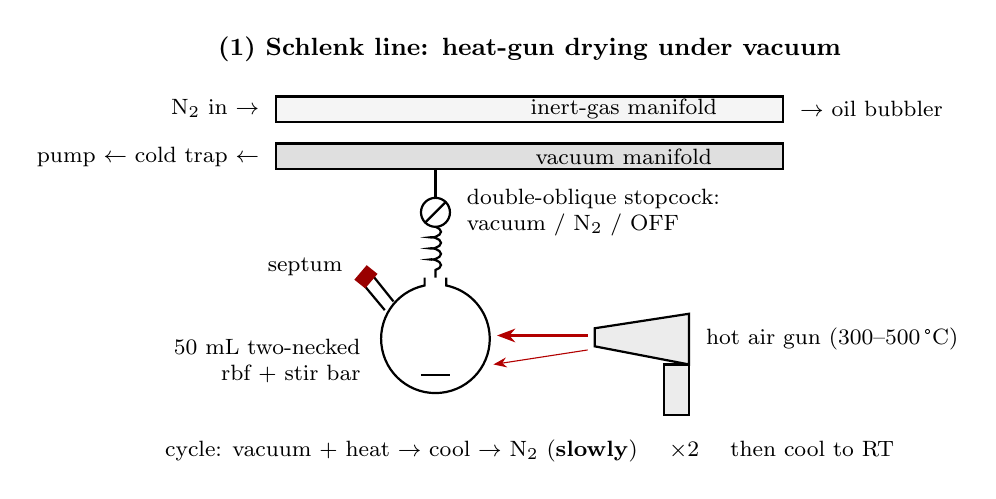
\begin{tikzpicture}[scale=0.92,font=\footnotesize]
  \node[font=\bfseries\small] at (3.5,5.2) {(1) Schlenk line: heat-gun drying under vacuum};
  \draw[thick,fill=gray!8] (0,4.2) rectangle (7,4.55);
  \draw[thick,fill=gray!25] (0,3.55) rectangle (7,3.9);
  \node[anchor=east] at (-0.1,4.38) {N$_2$ in $\to$};
  \node[anchor=west] at (7.1,4.38) {$\to$ oil bubbler};
  \node[anchor=east] at (-0.1,3.72) {pump $\leftarrow$ cold trap $\leftarrow$};
  \node at (4.8,4.38) {inert-gas manifold};
  \node at (4.8,3.72) {vacuum manifold};
  % stopcock
  \draw[thick] (2.2,3.55) -- (2.2,3.15);
  \draw[thick,fill=white] (2.2,2.95) circle (0.2);
  \draw[thick] (2.05,2.8) -- (2.35,3.1);
  \node[anchor=west,align=left] at (2.5,2.95) {double-oblique stopcock:\\ vacuum / N$_2$ / OFF};
  \draw[thick,decorate,decoration={coil,aspect=0.4,segment length=4pt,amplitude=2pt}] (2.2,2.75) -- (2.2,2.05);
  % flask: centre (2.2,1.2), r 0.75
  \draw[thick] (2.05,2.05) -- (2.05,1.94) arc[start angle=101.5,end angle=438.5,radius=0.75] -- (2.35,2.05);
  \draw[thick] (1.62,1.72) -- (1.3,2.12);
  \draw[thick] (1.5,1.6) -- (1.15,2.02);
  \fill[red!60!black] (1.08,2.02) -- (1.25,2.22) -- (1.4,2.1) -- (1.23,1.9) -- cycle;
  \node[anchor=east] at (1.05,2.2) {septum};
  \draw[thick] (2.0,0.7) -- (2.4,0.7);
  \node[anchor=east,align=right] at (1.3,0.9) {50 mL two-necked\\ rbf + stir bar};
  % heat gun
  \draw[thick,fill=gray!15] (4.4,1.1) -- (5.7,0.85) -- (5.7,1.55) -- (4.4,1.35) -- cycle;
  \draw[thick,fill=gray!15] (5.35,0.85) rectangle (5.7,0.15);
  \draw[-{Stealth},red!70!black,thick] (4.3,1.25) -- (3.05,1.25);
  \draw[-{Stealth},red!70!black] (4.3,1.05) -- (3.0,0.85);
  \node[anchor=west] at (5.8,1.2) {hot air gun (300--500\,°C)};
  \node[anchor=north,align=center] at (3.5,-0.05) {cycle: vacuum + heat $\to$ cool $\to$ N$_2$ (\textbf{slowly}) \quad $\times$2 \quad then cool to RT};
\end{tikzpicture}

\vspace{10pt}
% ---------- Panel 2 and 3 ----------
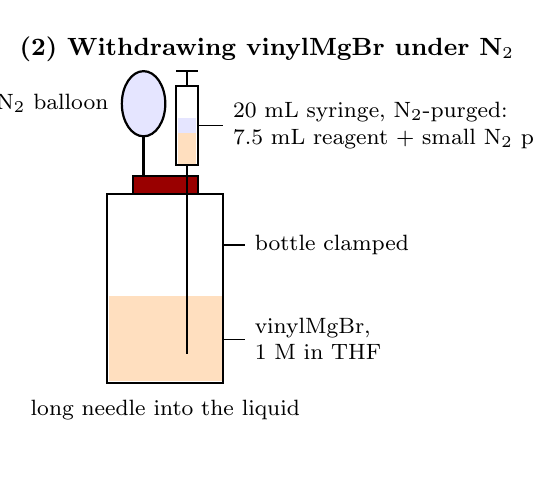
\begin{tikzpicture}[scale=0.92,font=\footnotesize]
  \useasboundingbox (-0.3,-1.0) rectangle (6.3,4.9);
  \node[font=\bfseries\small] at (3.0,4.6) {(2) Withdrawing vinylMgBr under N$_2$};
  \draw[thick,fill=white] (0.8,0) rectangle (2.4,2.6);
  \fill[orange!25] (0.82,0.02) rectangle (2.38,1.2);
  \draw[thick,fill=red!60!black] (1.15,2.6) rectangle (2.05,2.85);
  % balloon
  \draw[thick] (1.3,2.85) -- (1.3,3.4);
  \draw[thick,fill=blue!10] (1.3,3.85) ellipse (0.3 and 0.45);
  \node[anchor=east] at (0.95,3.85) {N$_2$ balloon};
  % syringe
  \draw[thick] (1.9,0.4) -- (1.9,3.0);
  \draw[thick,fill=white] (1.75,3.0) rectangle (2.05,4.1);
  \fill[orange!25] (1.77,3.02) rectangle (2.03,3.45);
  \fill[blue!10] (1.77,3.45) rectangle (2.03,3.65);
  \draw[thick] (1.9,4.1) -- (1.9,4.3) (1.75,4.3) -- (2.05,4.3);
  \draw (2.05,3.55) -- (2.4,3.55) node[anchor=west,align=left] {20 mL syringe, N$_2$-purged:\\ 7.5 mL reagent + small N$_2$ plug};
  \draw (2.4,0.6) -- (2.7,0.6) node[anchor=west,align=left] {vinylMgBr,\\ 1 M in THF};
  \draw (2.4,1.9) -- (2.7,1.9) node[anchor=west] {bottle clamped};
  \node[anchor=north] at (1.6,-0.1) {long needle into the liquid};
\end{tikzpicture}
\hfill
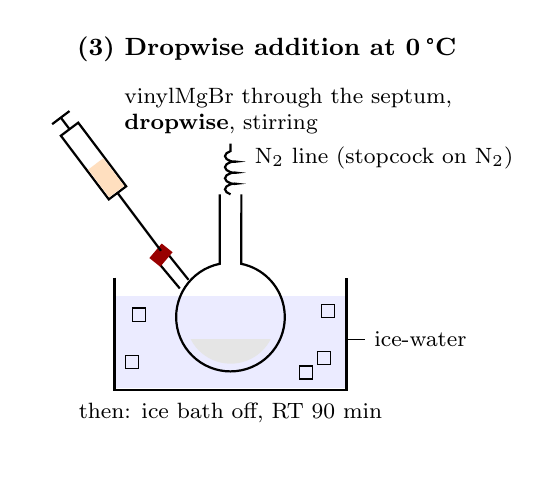
\begin{tikzpicture}[scale=0.92,font=\footnotesize]
  \useasboundingbox (-0.3,-1.0) rectangle (6.3,4.9);
  \node[font=\bfseries\small] at (3.0,4.6) {(3) Dropwise addition at 0\,°C};
  % ice bath
  \draw[thick] (0.9,1.45) -- (0.9,-0.1) -- (4.1,-0.1) -- (4.1,1.45);
  \fill[blue!8] (0.92,-0.08) rectangle (4.08,1.2);
  \foreach \x/\y in {1.05/0.2,1.15/0.85,3.7/0.25,3.75/0.9,3.45/0.05} \draw (\x,\y) rectangle ++(0.18,0.18);
  \draw (4.1,0.6) -- (4.35,0.6) node[anchor=west] {ice-water};
  % flask centre (2.5,0.9)
  \draw[thick] (2.35,2.6) -- (2.35,1.64) arc[start angle=101.5,end angle=438.5,radius=0.75] -- (2.65,2.6);
  \fill[gray!20] (1.95,0.6) arc[start angle=207,end angle=333,radius=0.62] -- cycle;
  \draw[thick] (1.92,1.42) -- (1.6,1.82);
  \draw[thick] (1.8,1.3) -- (1.45,1.72);
  \fill[red!60!black] (1.38,1.72) -- (1.55,1.92) -- (1.7,1.8) -- (1.53,1.6) -- cycle;
  \draw[thick,decorate,decoration={coil,aspect=0.4,segment length=4pt,amplitude=2pt}] (2.5,2.6) -- (2.5,3.3);
  \node[anchor=west] at (2.7,3.1) {N$_2$ line (stopcock on N$_2$)};
  % syringe: needle from septum (1.54,1.82) toward upper left
  \draw[thick] (1.54,1.82) -- (0.94,2.62);
  \begin{scope}[shift={(0.94,2.62)},rotate=37]
    \draw[thick,fill=white] (-0.15,0) rectangle (0.15,1.1);
    \fill[orange!25] (-0.13,0.02) rectangle (0.13,0.5);
    \draw[thick] (0,1.1) -- (0,1.3) (-0.15,1.3) -- (0.15,1.3);
  \end{scope}
  \node[anchor=west,align=left] at (0.9,3.75) {vinylMgBr through the septum,\\ \textbf{dropwise}, stirring};
  \node[anchor=north,align=center] at (2.5,-0.15) {then: ice bath off, RT 90 min};
\end{tikzpicture}

\vspace{10pt}
% ---------- Panel 4: extraction ----------
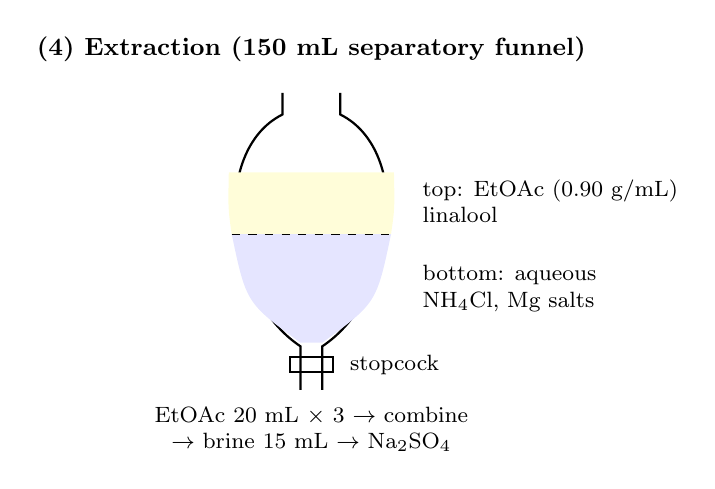
\begin{tikzpicture}[scale=0.92,font=\footnotesize]
  \node[font=\bfseries\small] at (2.0,5.0) {(4) Extraction (150 mL separatory funnel)};
  \draw[thick] (1.6,4.4) -- (1.6,4.1) .. controls (0.6,3.6) and (0.8,1.6) .. (1.85,0.9) -- (1.85,0.3);
  \draw[thick] (2.4,4.4) -- (2.4,4.1) .. controls (3.4,3.6) and (3.2,1.6) .. (2.15,0.9) -- (2.15,0.3);
  \fill[yellow!15] (0.86,3.3) -- (3.14,3.3) .. controls (3.15,2.8) .. (3.1,2.45) -- (0.9,2.45) .. controls (0.85,2.8) .. cycle;
  \fill[blue!10] (0.9,2.45) -- (3.1,2.45) .. controls (2.9,1.5) .. (2.15,0.95) -- (1.85,0.95) .. controls (1.1,1.5) .. cycle;
  \draw[dashed] (0.9,2.45) -- (3.1,2.45);
  \draw[thick] (1.7,0.55) rectangle (2.3,0.75);
  \node[anchor=west,align=left] at (3.4,2.9) {top: EtOAc (0.90 g/mL)\\ linalool};
  \node[anchor=west,align=left] at (3.4,1.7) {bottom: aqueous\\ NH$_4$Cl, Mg salts};
  \node[anchor=west] at (2.4,0.65) {stopcock};
  \node[anchor=north,align=center] at (2.0,0.2) {EtOAc 20 mL $\times$ 3 $\to$ combine\\ $\to$ brine 15 mL $\to$ Na$_2$SO$_4$};
\end{tikzpicture}
\hspace{0.8cm}
\begin{minipage}[b]{7.2cm}
\small
\textbf{Stopcock positions (two-way valve)}\par\smallskip
{\renewcommand{\arraystretch}{1.4}
\begin{tabularx}{\linewidth}{|l|Y|}
\hline
\textbf{Vacuum} & flask open to the pump: drying cycles\\ \hline
\textbf{N$_2$} & flask open to inert gas: backfill (slowly), during the reaction\\ \hline
\textbf{OFF} & flask isolated: before disconnecting for work-up\\ \hline
\end{tabularx}}
\vspace{18pt}
\end{minipage}
\end{center}

\begin{tcolorbox}[safety,title={ORDER OF EVENTS}]
\small
Hood cleared $\to$ vacuum + heat gun $\to$ cool $\to$ N$_2$ (\textbf{slowly}) $\times$2 $\to$ RT $\to$ ketone + THF $\to$ ice bath 5--10 min $\to$ vinylMgBr 7.5 mL \textbf{dropwise} $\to$ RT \textbf{90 min} (quench syringe, pre-weigh rbf, set up TLC) $\to$ valve OFF, disconnect $\to$ ice bath, \textbf{vent}, sat.\ NH$_4$Cl dropwise $\to$ water $\to$ EtOAc $\times$3 $\to$ brine $\to$ Na$_2$SO$_4$ 15 min + \textbf{TLC} $\to$ filter $\to$ rotavap $\to$ \textbf{weigh crude} $\to$ store for Week 11.\\
\textbf{Tip (not in the manual).} If the Grignard reagent looks cloudy or has a solid at the bottom of the bottle, tell the GTA before drawing it: a precipitate can mean partial hydrolysis, and less active reagent shows up as unreacted ketone on the TLC.
\end{tcolorbox}

\end{document}
